\documentclass[11pt,aspectratio=169]{beamer}

%\mode<handout>
%{
	%	\usepackage{pgf}
	%	\usepackage{pgfpages}
	%	
	%	\pgfpagesdeclarelayout{4 on 1 boxed}
	%	{
		%		\edef\pgfpageoptionheight{\the\paperheight} 
		%		\edef\pgfpageoptionwidth{\the\paperwidth}
		%		\edef\pgfpageoptionborder{0pt}
		%	}
	%	{
		%		\pgfpagesphysicalpageoptions
		%		{%
			%			logical pages=4,%
			%			physical height=\pgfpageoptionheight,%
			%			physical width=\pgfpageoptionwidth%
			%		}
		%		\pgfpageslogicalpageoptions{1}
		%		{%
			%			border code=\pgfsetlinewidth{2pt}\pgfstroke,%
			%			border shrink=\pgfpageoptionborder,%
			%			resized width=.5\pgfphysicalwidth,%
			%			resized height=.5\pgfphysicalheight,%
			%			center=\pgfpoint{.25\pgfphysicalwidth}{.75\pgfphysicalheight}%
			%		}%
		%		\pgfpageslogicalpageoptions{2}
		%		{%
			%			border code=\pgfsetlinewidth{2pt}\pgfstroke,%
			%			border shrink=\pgfpageoptionborder,%
			%			resized width=.5\pgfphysicalwidth,%
			%			resized height=.5\pgfphysicalheight,%
			%			center=\pgfpoint{.75\pgfphysicalwidth}{.75\pgfphysicalheight}%
			%		}%
		%		\pgfpageslogicalpageoptions{3}
		%		{%
			%			border code=\pgfsetlinewidth{2pt}\pgfstroke,%
			%			border shrink=\pgfpageoptionborder,%
			%			resized width=.5\pgfphysicalwidth,%
			%			resized height=.5\pgfphysicalheight,%
			%			center=\pgfpoint{.25\pgfphysicalwidth}{.25\pgfphysicalheight}%
			%		}%
		%		\pgfpageslogicalpageoptions{4}
		%		{%
			%			border code=\pgfsetlinewidth{2pt}\pgfstroke,%
			%			border shrink=\pgfpageoptionborder,%
			%			resized width=.5\pgfphysicalwidth,%
			%			resized height=.5\pgfphysicalheight,%
			%			center=\pgfpoint{.75\pgfphysicalwidth}{.25\pgfphysicalheight}%
			%		}%
		%	}
	%	
	%	
	%	\pgfpagesuselayout{4 on 1 boxed}[a4paper, border shrink=5mm, landscape]
	%	\nofiles
	%}
\usefonttheme[onlymath]{serif}
\usetheme[outer/progressbar=foot,
%outer/numbering=none
]{metropolis}
\setbeamertemplate{caption}{\raggedright\insertcaption\par}
\setbeamercolor{frametitle}{bg={}, fg=black!80}
\definecolor{myorange}{rgb}{0.8500, 0.3250, 0.0980}
\setbeamercolor{alerted text}{bg={}, fg=myorange }
\setbeamercolor{block title}{bg=black!10, fg=black}
\setbeamercolor{block body}{bg=black!10, fg=black}
\setbeamercolor{block frame}{bg=black, fg=black}
\setbeamertemplate{blocks}[rounded]
\setbeamertemplate{blocks}[framed]
%\usecolortheme{seahorse}
\usepackage[utf8]{inputenc}
\usepackage[english]{babel}
%\usepackage[T1]{fontenc}
\newcommand{\tr}[1]{\textcolor{blue}{#1}}
\usepackage{amsmath}
\usepackage{amsfonts}
\usepackage{amssymb}
\usepackage{mathtools}
\usepackage{calc}
\usepackage{soul}
\setbeamercolor{headerCol}{fg=blue!30,bg=black!80}
\setbeamercolor{bodyCol}{fg=black}
\usepackage{graphicx}
\usepackage{xcolor}
\usepackage{appendix}
\usepackage{hyperref}
\usepackage{natbib}
\usepackage{comment}
\usepackage{setspace}
\renewcommand{\bibsection}{}
\bibliographystyle{apa} 
% have to run bibtex mydocument.aux after first run to generate bbl file. 
\usepackage{appendixnumberbeamer}
\usepackage{xcolor}
\usepackage{subcaption}
%table
\usepackage{makecell}
\usepackage{multirow}
\usepackage{bigdelim}

\newif\ifabbreviation
\pretocmd{\thebibliography}{\abbreviationfalse}{}{}
\AtBeginDocument{\abbreviationtrue}
\DeclareRobustCommand\acroauthor[2]{%
	\ifabbreviation #2\else #1 (\mbox{#2})\fi}

\usepackage[customcolors]{hf-tikz}
\definecolor{sonja}{cmyk}{1.5,0,0.9,0.3}
%\definecolor{blue}{cmyk}{0,1,0,0}
\hfsetfillcolor{black!10}
\hfsetbordercolor{black}

\usepackage{tikz}
\usetikzlibrary{tikzmark}
\newcommand{\ImageWidth}{11cm}
\usetikzlibrary{decorations.pathreplacing,positioning, arrows.meta}
\usetikzlibrary{decorations.markings}
\usepackage{tikz-cd}
\usetikzlibrary{arrows,calc,fit}
\tikzset{mainbox/.style={draw=white, text=white, fill=gray, rectangle, rounded corners, thick, node distance=7em, text width=8em, text centered, minimum height=3.5em}}
\tikzset{dummybox/.style={draw=none, text=white , rectangle, rounded corners, thick, node distance=7em, text width=8em, text centered, minimum height=3.5em}}
\tikzset{box/.style={draw , rectangle, rounded corners, thick, node distance=7em, text width=8em, text centered, minimum height=3.5em}}
\tikzset{container/.style={draw, rectangle, dashed, inner sep=2em}}
\tikzset{line/.style={draw, very thick, -latex'}}
\tikzset{    pil/.style={
		->,
		thick,
		shorten <=2pt,
		shorten >=2pt,}}
\tikzstyle{vecArrow} = [thick, decoration={markings,mark=at position
	1 with {\arrow[semithick]{open triangle 60}}},
double distance=1.4pt, shorten >= 5.5pt,
preaction = {decorate},
postaction = {draw,line width=1.4pt, white,shorten >= 4.5pt}]
\usetikzlibrary{shapes}
\renewcommand{\figurename}{}

%TITLE
\author[Sonja Dobkowitz]{\small Sonja Dobkowitz\\ \footnotesize{University of Bonn%, RTG 2281 The Macroeconomics of Inequality}
}\\ }
%\institute[University of Bonn]{}
\title{Meeting Climate Targets: The Optimal Fiscal Policy Mix}

\newcommand{\ar}{$\Rightarrow$ \ }

%\addtobeamertemplate{navigation symbols}{}{%
%    \usebeamerfont{footline}%
%    \usebeamercolor[fg]{footline}%
%    \hspace{1em}%
%   \insertframenumber/\inserttotalframenumber
%}

%\institute{University of Bonn} 
\date{\small{Presentation at Trinity College Dublin\\ January 27, 2023 }} 
%\subject{} 
\begin{document}

\tikzstyle{modus}=[rectangle,inner sep=5mm,align=center, draw]
\tikzstyle{dialog}=[diamond, align=center, draw]
\tikzstyle{sphere}=[circle, align=center, dotted, minimum size=3cm, draw]
\tikzstyle{circll}=[circle, align=center, minimum size=3cm, draw]
\tikzstyle{circllsmall}=[circle, align=center, minimum size=2cm, draw]
{\setbeamertemplate{footline}{}
	\begin{frame}
		\titlepage
	\end{frame}
}
%\addtocounter{framenumber}{-1}

% {\setbeamertemplate{footline}{}
	% \begin{frame}{Content}
		% \vspace{4mm}
		% \tableofcontents
		% \end{frame}
	% }
%\addtocounter{framenumber}{-1}


%---------------------------------------
%            Intro
%---------------------------------------
\addtocounter{framenumber}{-1}
\begin{frame}{Motivation}
	\begin{itemize}[<+-| alert@+>]
		\setbeamercolor{alerted text}{} %change the font color
		\setbeamerfont{alerted text}{}
		\item How to best meet emission targets in line with climate goals? % Frage
		\vspace{3mm}
		\item Problem:
		\begin{itemize}
			\item[-] On the one hand,  reduce the use of fossil fuels,...
			\vspace{2mm}
			\item[-] ... on the other hand, %keep research productivity high 
			maintain some fossil research activity 
			\vspace{1mm}
			\begin{enumerate}
				\item[-] research in established sectors more productive
				%\item[-] higher risk of duplicating ideas if all research happens in one sector
				\item[-] non-green knowledge facilitates green innovation tomorrow %\tiny{\citep{Barbieri2021GreenPolicy}}
			\end{enumerate}% idea that researchers learn from past findings: building on the shoulder of giants mechanism
			%				and 
			\vspace{2mm}				
			\item[-] A \textbf{carbon tax} lowers the use fossil fuels but also reduces research in established industries %state of the art
		\end{itemize} 
		\vspace{3mm}
		\item My contribution: discuss \textbf{labor income taxes} as a potential solution
		\vspace{3mm}
		\item[] \hspace{-4mm}\alert{{What is the optimal mix of carbon and labor income taxes to meet emission targets?}}
	\end{itemize}
\end{frame}


\begin{comment}
\addtocounter{framenumber}{-1}
\begin{frame}{Motivation}
	
	\begin{itemize}[<+-| alert@+>]
		\setbeamercolor{alerted text}{} %change the font color
		\setbeamerfont{alerted text}{}
		%	\item we are facing  environmental limits 
		%	\vspace{3mm}
		\item meeting climate targets requires a limit on emissions \citep{IPCC2022}
		\vspace{3mm}
		\item carbon taxes  direct  (i) demand towards emission-low alternatives\\ \hspace{23mm} \underline{and} (ii) research across sectors
		\vspace{3mm}
		\item labor income taxes affect the level of production 
		\vspace{3mm}
		\item \textbf{What is the optimal policy mix to meet the emission target?}
	\end{itemize}
\end{frame}


content...

\begin{frame}{This paper}
	\vspace{-2mm}
	\begin{itemize}
		\item<+-> quantitative model of \alert{directed technical change} building on \cite{Fried2018ClimateAnalysis}
		\vspace{2mm}
		\item<+->   the government   chooses the \alert{path of carbon and income taxes} to maximize welfare\vspace{2mm}
		\item<+-> an \alert{emission limit} constrains the government
	\end{itemize}
	\pause
	\begin{center}
		\begin{figure}
			\centering
			\textbf{US net CO$_2$ emission limit in Gt}\\
			\vspace{2mm}	\includegraphics[width=0.38\textwidth]{../codding_model/own_basedOnFried/optimalPol_010922_revision/figures/all_13Sept22_Tplus30/Emnet.png}
		\end{figure}
	\end{center}
\end{frame}
\end{comment}

\begin{frame}{This paper}
	\vspace{-4mm}
	\begin{itemize}
		\item<+-> Quantitative model building on \cite{Fried2018ClimateAnalysis} 
		\vspace{2mm}
		\begin{itemize}
			\item[-]<+-> \alert{technologies are sector specific}: green, fossil, and non-energy sector 
			\vspace{1mm}
			\item[-]<+-> \alert{research} on technologies augments productivity within a sector \\ \footnotesize{(directed technical change) }
			\vspace{1mm}
			\item[-]<+-> \alert{knowledge spillovers}: 
			\begin{enumerate}
				\item[a)]<+-> \alert{within-sector}: researchers learn from knowledge accumulated in their sector
				\item[b)]<+-> \alert{cross-sector}: knowledge generated in sector A stimulates innovation in sector B
			\end{enumerate}%\\ \footnotesize{(cross-sectoral knowledge spillovers)}
		\end{itemize}
		\vspace{2mm}
		\item<+->   The government   chooses the \alert{path of carbon and income taxes} to maximize welfare\vspace{2mm}
		\item<+-> An \alert{emission limit} constrains the government: 
		%		\begin{itemize}
			%			\item[-]<+-> positive net emissions before 2050
			%			\item[-]<+-> net-zero emissions from 2050 onward
			%		\end{itemize}
	\end{itemize}
	\pause
	\vspace{0mm}
	\centering
	\resizebox{290pt}{70pt}{%
		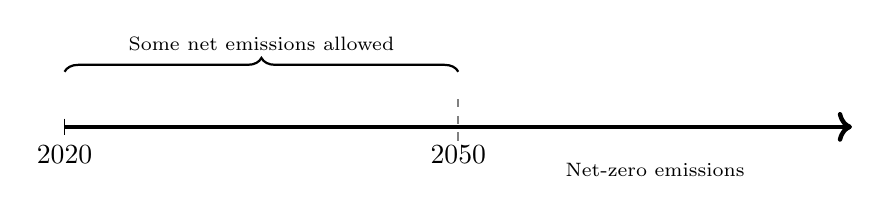
\begin{tikzpicture}
			\draw[ultra thick, ->] (0,0) -- (10,0);
			\foreach \x in {0}
			\draw (\x cm,3pt) -- (\x cm,-3pt);
			\foreach \x in {5}
			\draw[dashed, gray, thick] (\x cm,10pt) -- (\x cm,-6pt);
			% draw node
			\draw[thick] (0,0) node[below=3pt,thick] {2020} node[above=3pt] {};
			\draw[thick] (5,0) node[below=3pt,thick] {2050} node[above=3pt] {};
			\draw [thick ,decorate,decoration={brace,amplitude=5pt}] (0,0.7)  -- +(5,0) 
			node [black,midway,above=4pt, font=\scriptsize] {Some net emissions allowed};
			\node[draw=none, black, above=4pt, font=\scriptsize] (B1) at (7.5,-.9) {Net-zero emissions};
			
		\end{tikzpicture}
	}
	%	\pause
	%	\begin{center}
		%		\begin{figure}
			%	\caption{US CO$_2$ emission limit in Gt}
			%	\vspace{-2mm}
			%	\includegraphics[width=0.4\textwidth]{../codding_model/own_basedOnFried/optimalPol_010922_revision/figures/all_13Sept22_Tplus30/Emnet_goals_o0_lgd0.png}
			%\end{figure}
			%	\end{center}
	\end{frame}
	
	
	\begin{frame}{Preview of results}
		\centering
		\vspace{-3mm}
		\begin{itemize}[<+-| alert@+>]
			\setbeamercolor{alerted text}{} %change the font color
			\setbeamerfont{alerted text}{}
			%begin{minipage}[]{1\textwidth}
			%\begin{itemize}
			\item A combination of carbon and labor income taxes is optimal to target the direction of research
			\vspace{3mm}
			\item Before the net-zero emission limit (ca. 2020-2050): 
			\begin{itemize}
				\item[-] lower carbon tax to maintain some fossil research %\tr{give an example of knowledge spillovers here}
				\item[-] a tax on labor reduces emissions
			\end{itemize}
			\vspace{3mm}
			\item Under the net-zero emission limit (from 2050 onward): 
			\begin{itemize}
				\item[-]  higher carbon tax to foster green research
				\item[-]  a smaller tax on labor boosts output
			\end{itemize}
			\vspace{3mm}
			\item Limited use of labor income tax \ar look at research subsidies
			%		\begin{itemize}
				%			\item[-] income tax remains beneficial to correct labor market distortions arising from lack of lump-sum rebates of carbon tax revenues
				%			%\item[-] when only green research subsidies are available, welfare smaller than with lump-sum rebates			
				%		\end{itemize}
			%; \tr{e.g. a higher marginal value of leisure}	%	\end{minipage}
	\end{itemize}
\end{frame}

\begin{comment}
	\begin{frame}
		\begin{itemize}
			\item How to best implement emission targets in line with climate goals?
			\item 2 adjustment possibilities to reduce emissions: 
			\begin{enumerate}
				\item shift from fossil to green production technologies (e.g. carbon tax, green subsidies)
				\item lower the level of production overall (e.g. labor income taxes)
			\end{enumerate}
			\item Literature focuses on 1st point
		\end{itemize}
	\end{frame}
\end{comment}

\begin{frame}{Contribution to the literature}
	\begin{itemize}[<+->]
		\item \alert{\textbf{Standard to have inelastic labor supply in environmental policy discussion}}\\  \footnotesize{ \citep{Acemoglu2012TheChange, Golosov2014OptimalEquilibrium, Acemoglu2016TransitionTechnology, Fried2018ClimateAnalysis, Hart2019TheEconomists}}
		\\  \normalsize{\alert{\ar precludes studying combinations of policies targeted at the composition and\\ \hspace{5mm} the level of production }}
		\vspace{2mm}
		\item \alert{Labor income taxes and environmental policies in the literature}
		\begin{itemize}
			\item[-]  government funding condition; generally passive \footnotesize{ \citep{ LansBovenberg1994EnvironmentalTaxation, Goulder1995EnvironmentalGuide, Barrage2019OptimalPolicy}} % Not an env. policy instrument
			\item[-] labor income taxes arise as environmental policy tool due to {income inequality} \footnotesize{\citep{Jacobs2019RedistributionCurves, Dobkowitz2022, Douenne2022OptimalHouseholds}}
			%	\item[-] This paper: novel motive for the use of labor income taxes within the optimal environmental policy: endogeneity of the allocation of researchers
		\end{itemize}		
		% Das klingt gut (differenzierung zwischen wirkungsweisen und nicht instrumenten! ): weil instrumente beide effekte haben können, dass die carbon tax auch das level beeinflusst wird ausgeklammert
		% I argue that we should study optimal env. policies allowing for level adjustments of production! I provide am example scenario where adjusting the level becomes part of the optimal policy
		\vspace{2mm}
		\item \alert{This paper}: motive for labor income taxation solely arises from environmental externality % alone %directly % is optimal due to  directed technical change % and (ii) lack of research subsidies
		%	\footnotesize{\citep{Acemoglu2012TheChange}}
		%\\ \normalsize{\alert{\ar role for labor income taxation}}
		% weak double dividend literature (advantage to use env tac revenues to lower existing distortions; deviation of optimal env tax from pigou)
		%			\begin{itemize}
			%			%	\item[-] Research subsidies essential to implement first best.
			%			%	Otherwise, carbon tax higher to bolster green research; costly in terms of output
			%			%	\item[-]  In this case, labor income taxes may help get closer to first best
			%				\item[-] I add a richer, quantitative framework \ar new qualitative insights % increasing carbon tax, potentially fossil subsidy optimal
			%				\item[-]  insights on importance of additional measures
			%			\end{itemize}
		%	With knowledge spillovers \ar (i) increasing policy intervention, (ii) potentially advantageous to maintain some fossil research
		%	\vspace{2mm}
		%	% theirs is an analytical model; qualitative results; I look at a quantitative framework
		%	\item Quantitative framework builds on \cite{Fried2018ClimateAnalysis} %\ar new qualitative insights
		%	\begin{itemize}
			%		\item[-] I add a \alert{dynamic optimal policy analysis} under an exogenous \alert{dynamic emission target} %eventually declining to \alert{net-zero emissions}
			%		\item[-] \alert{elastic labor supply}
			%	\end{itemize}
	\end{itemize}
\end{frame}


\section{Model and Mechanisms}
\begin{frame}{Model}
	\begin{figure}[h]
		%	\vspace{-4mm}
		\centering
		\begin{tikzpicture}[auto,scale=.7, transform shape]
			
			\node[circll] (A) at (-7,4)  {\textbf{{\hyperlink{prodmod}{Production}}}\\ \textbf{{and Research}}};
			\node[circll] (B) at (7,4) {\textbf{\hyperlink{backhh}{{Representative}}}\\ \textbf{\hyperlink{backhh}{{Household}}}};
			\node[circll] (D) at (0,9) {\textbf{Government}};
		\end{tikzpicture}
	\end{figure}
\end{frame}

\addtocounter{framenumber}{-1}
\begin{frame}{Model}
	\begin{figure}[h]
		\vspace{-4mm}
		\centering
		\begin{tikzpicture}[auto,scale=.7, transform shape]
			\node[circll] (A) at (-7,4) {\textbf{{\hyperlink{prodmod}{Production}}}\\ \textbf{{and Research}}};
			\node[circll] (B) at (7,4) {\textbf{\hyperlink{backhh}{{Representative}}}\\ \textbf{\hyperlink{backhh}{{Household}}}};
			\node[circll] (D) at (0,9) {\textbf{Government}}; 
			
			\node[draw=none] (B1) at (5,4.25) {};
			\node[draw=none] (B2) at (5,3.5) {};
			\node[draw=none] (BA1) at (-5,4.25) {};
			\node[draw=none] (BA2) at (-5,3.5) {};
			\node[draw=none] (D1) at (1.8,7.8) {};
			
			\node[draw=none] (B22) at (6.4,5.6) {};
			\node[draw=none] (D2) at (2.3,8.5) {};
			\node[draw=none] (B3) at (5.3,5.3) {};
			\node[draw=none] (D3) at (-1.5,7) {};
			\node[draw=none] (A1) at (-4.2,4.6) {};
			
			
			
			\draw [->] (B1) to node[pos=0.75, swap]{Workers and scientists} (BA1);
			\draw [->] (BA2) to node[pos=0.75, swap]{Final good} (B2);
		\end{tikzpicture}
		
	\end{figure}
\end{frame}
\addtocounter{framenumber}{-1}
\begin{frame}{Model}
	\begin{figure}[h]
		\vspace{-4mm}
		\centering
		\begin{tikzpicture}[auto,scale=.7, transform shape]
			\node[circll] (A) at (-7,4) {\textbf{{\hyperlink{prodmod}{Production}}}\\ \textbf{{and Research}}};
			\node[circll] (B) at (7,4) {\textbf{\hyperlink{backhh}{{Representative}}}\\ \textbf{\hyperlink{backhh}{{Household}}}};
			\node[circll] (D) at (0,9) {\textbf{\alert{Government}}\\ \textbf{max welfare} \\ \textbf{s.t. emission limit} }; 
			\node[draw=none] (B1) at (5,4.25) {};
			\node[draw=none] (B2) at (5,3.5) {};
			\node[draw=none] (BA1) at (-5,4.25) {};
			\node[draw=none] (BA2) at (-5,3.5) {};
			\node[draw=none] (D1) at (1.8,7.8) {};
			
			\node[draw=none] (B22) at (6.4,5.6) {};
			\node[draw=none] (D2) at (2.3,8.5) {};
			\node[draw=none] (B3) at (5.3,5.3) {};
			\node[draw=none] (D3) at (-1.5,7) {};
			\node[draw=none] (A1) at (-4.2,4.6) {};
			\node[draw=none] (D4) at (-2,8.3) {};
			\node[draw=none] (A4) at (-6,5.4) {};
			%\draw [->] (B22) to node[pos=0.5, swap]{\alert{Tax on labor, $\pmb{\tau_{\iota}}$}} (D2);
			%\draw [->] (D1) to node[pos=0.5, swap]{Transfers} (B3);
			
			\draw [->] (B1) to node[pos=0.75, swap]{Workers and scientists} (BA1);
			\draw [->] (BA2) to node[pos=0.75, swap]{Final good} (B2);
			%	\draw [->] (A4) to node[pos=0.5, swap]{\alert{Tax on carbon, $\pmb{\tau_F}$}}   (D4);
		\end{tikzpicture}
		
	\end{figure}
\end{frame}

\addtocounter{framenumber}{-1}
\begin{frame}{Model}
	\begin{figure}[h]
		\vspace{-4mm}
		\centering
		\begin{tikzpicture}[auto,scale=.7, transform shape]
			\node[circll] (A) at (-7,4) {\textbf{{\hyperlink{prodmod}{Production}}}\\ \textbf{{and Research}}};
			\node[circll] (B) at (7,4) {\textbf{\hyperlink{backhh}{{Representative}}}\\ \textbf{\hyperlink{backhh}{{Household}}}};
			\node[circll] (D) at (0,9) {\textbf{\alert{Government}}\\ \textbf{max welfare} \\ \textbf{s.t. emission limit} }; 
			\node[draw=none] (B1) at (5,4.25) {};
			\node[draw=none] (B2) at (5,3.5) {};
			\node[draw=none] (BA1) at (-5,4.25) {};
			\node[draw=none] (BA2) at (-5,3.5) {};
			\node[draw=none] (D1) at (1.8,7.8) {};
			
			\node[draw=none] (B22) at (6.4,5.6) {};
			\node[draw=none] (D2) at (2.3,8.5) {};
			\node[draw=none] (B3) at (5.3,5.3) {};
			\node[draw=none] (D3) at (-1.5,7) {};
			\node[draw=none] (A1) at (-4.2,4.6) {};
			\node[draw=none] (D4) at (-2,8.3) {};
			\node[draw=none] (A4) at (-6,5.4) {};
			\draw [->] (B22) to node[pos=0.65, swap]{\alert{Tax on labor, $\pmb{\tau_{\iota}}$:}} (D2);
			\draw [->] (B22) to node[pos=0.45, swap]{\alert{$\pmb{\tau_{\iota}}>0$:  labor supply $\downarrow$ \ar emissions $\downarrow$}} (D2);
			%	\draw [->] (B22) to node[pos=0.3, swap]{\alert{$\pmb{\tau_{\iota}}<0$:    labor supply $\uparrow$ \ar output $\uparrow$}} (D2);
			\draw [->] (D1) to node[pos=0.5, swap]{Transfers} (B3);
			
			\draw [->] (B1) to node[pos=0.75, swap]{Workers and scientists} (BA1);
			\draw [->] (BA2) to node[pos=0.75, swap]{Final good} (B2);
			%	\draw [->] (A4) to node[pos=0.5, swap]{\alert{Tax on carbon, $\pmb{\tau_F}$}}   (D4);
		\end{tikzpicture}
		
	\end{figure}
\end{frame}

\addtocounter{framenumber}{-1}
\begin{frame}{Model}
	\begin{figure}[h]
		\vspace{-4mm}
		\centering
		\begin{tikzpicture}[auto,scale=.7, transform shape]
			\node[circll] (A) at (-7,4) {\textbf{{\hyperlink{prodmod}{Production}}}\\ \textbf{{and Research}}};
			\node[circll] (B) at (7,4) {\textbf{\hyperlink{backhh}{{Representative}}}\\ \textbf{\hyperlink{backhh}{{Household}}}};
			\node[circll] (D) at (0,9) {\textbf{\alert{Government}}\\ \textbf{max welfare} \\ \textbf{s.t. emission limit} }; 
			\node[draw=none] (B1) at (5,4.25) {};
			\node[draw=none] (B2) at (5,3.5) {};
			\node[draw=none] (BA1) at (-5,4.25) {};
			\node[draw=none] (BA2) at (-5,3.5) {};
			\node[draw=none] (D1) at (1.8,7.8) {};
			
			\node[draw=none] (B22) at (6.4,5.6) {};
			\node[draw=none] (D2) at (2.3,8.5) {};
			\node[draw=none] (B3) at (5.3,5.3) {};
			\node[draw=none] (D3) at (-1.5,7) {};
			\node[draw=none] (A1) at (-4.2,4.6) {};
			\node[draw=none] (D4) at (-2,8.3) {};
			\node[draw=none] (A4) at (-6,5.4) {};
			\draw [->] (B22) to node[pos=0.65, swap]{\alert{Tax on labor, $\pmb{\tau_{\iota}}$:}} (D2);
			\draw [->] (B22) to node[pos=0.45, swap]{\alert{$\pmb{\tau_{\iota}}>0$:  labor supply $\downarrow$ \ar emissions $\downarrow$}} (D2);
			\draw [->] (B22) to node[pos=0.3, swap]{\alert{$\pmb{\tau_{\iota}}<0$:    labor supply $\uparrow$ \ar output $\uparrow$}} (D2);
			\draw [->] (D1) to node[pos=0.5, swap]{Transfers} (B3);
			
			\draw [->] (B1) to node[pos=0.75, swap]{Workers and scientists} (BA1);
			\draw [->] (BA2) to node[pos=0.75, swap]{Final good} (B2);
			%	\draw [->] (A4) to node[pos=0.5, swap]{\alert{Tax on carbon, $\pmb{\tau_F}$}}   (D4);
		\end{tikzpicture}
		
	\end{figure}
\end{frame}

\addtocounter{framenumber}{-1}
\begin{frame}{Model}
	\begin{figure}[h]
		\vspace{-4mm}
		\centering
		\begin{tikzpicture}[auto,scale=.7, transform shape]
			\node[circll] (A) at (-7,4) {\textbf{{\hyperlink{prodmod}{Production}}}\\ \textbf{{and Research}}};
			\node[circll] (B) at (7,4) {\textbf{\hyperlink{backhh}{{Representative}}}\\ \textbf{\hyperlink{backhh}{{Household}}}};
			\node[circll] (D) at (0,9) {\textbf{\alert{Government}}\\ \textbf{max welfare} \\ \textbf{s.t. Emission limit} }; 
			\node[draw=none] (B1) at (5,4.25) {};
			\node[draw=none] (B2) at (5,3.5) {};
			\node[draw=none] (BA1) at (-5,4.25) {};
			\node[draw=none] (BA2) at (-5,3.5) {};
			\node[draw=none] (D1) at (1.8,7.8) {};
			
			\node[draw=none] (B22) at (6.4,5.6) {};
			\node[draw=none] (D2) at (2.3,8.5) {};
			\node[draw=none] (B3) at (5.3,5.3) {};
			\node[draw=none] (D3) at (-1.5,7) {};
			\node[draw=none] (A1) at (-4.2,4.6) {};
			\node[draw=none] (D4) at (-2,8.3) {};
			\node[draw=none] (A4) at (-6,5.4) {};
			\draw [->] (B22) to node[pos=0.5, swap]{{Tax on labor, $\pmb{\tau_{\iota}}$}} (D2);
			\draw [->] (D1) to node[pos=0.5, swap]{Transfers} (B3);
			
			\draw [->] (B1) to node[pos=0.75, swap]{Workers and scientists} (BA1);
			\draw [->] (BA2) to node[pos=0.75, swap]{Final good} (B2);
			\draw [->] (A4) to node[pos=0.5, swap]{\alert{Tax on carbon, $\pmb{\tau_F}$}}   (D4);
		\end{tikzpicture}
		
	\end{figure}
\end{frame}
\begin{frame}{Production}
	\begin{figure}[h]
		\vspace{-10mm}
		\centering
		\begin{tikzpicture}[auto,scale=.7, transform shape]
			\node[circll] (A) at (0,17) {\textbf{Final}\textbf{ Good}}; 
			\node[circll] (B) at (-6,14) {\textbf{Energy}};
			\node[circll] (C) at (5,14) {\textbf{{Non-energy}}};
			\node[circll] (D) at (-10,12) {\textbf{{Fossil}}};
			\node[circll] (E) at (-2,12) {\textbf{{Green}}};
			\node[sphere] (Ems) at (-11,16) {\textbf{Emissions}};
			
			%		\node[circllsmall] (CM) at (4.6,8) {\textbf{{Machines}}};
			%		\node[circllsmall] (CL) at (7.4,8) {\textbf{{Labor}}};			\node[circllsmall] (EM) at (-3.4,8) {\textbf{{Machines}}};
			%	    \node[circllsmall] (EL) at (-0.6,8) {\textbf{{Labor}}};
			%	    \node[circllsmall] (DM) at (-11.4,8) {\textbf{{Machines}}};
			%	    \node[circllsmall] (DL) at (-8.6,8) {\textbf{{Labor}}};
			
			
			\draw [->] (B) to node[pos=0.5, swap]{} (A);
			\draw [->] (C) to node[pos=0.5, swap]{} (A);
			
			\draw [->] (E) to node[pos=0.5, swap]{} (B);
			\draw [->] (D) to node[pos=0.5, swap]{} (B);
			
			%		
			%		\draw [->] (EM) to node[pos=0.5, swap]{} (E);
			%		\draw [->] (EL) to node[pos=0.5, swap]{} (E);
			%		
			%		
			%		\draw [->] (DM) to node[pos=0.5, swap]{} (D);
			%		\draw [->] (DL) to node[pos=0.5, swap]{} (D);
			%		
			%		
			%		\draw [->] (CM) to node[pos=0.5, swap]{} (C);
			%		\draw [->] (CL) to node[pos=0.5, swap]{} (C);
			
			\draw [->] (D) to node[pos=0.5, swap]{} (Ems);
		\end{tikzpicture}
		
	\end{figure}
\end{frame}

\begin{frame}{1st: Effect of a carbon tax on \alert{fossil demand}}
	%	\begin{minipage}{0.4\textwidth}
		\begin{figure}[h]
			\vspace{-4mm}
			\centering
			\begin{tikzpicture}[auto,scale=.7, transform shape]
				%			\node[circll] (A) at (0,16) {\textbf{Final}\textbf{ Good}}; 
				\node[circll] (B) at (-6,14) {\textbf{Energy}};
				%			\node[circll] (C) at (5,14) {\textbf{{Non-energy}}};
				\node[circll] (D) at (-10,12) {\textbf{{Fossil}}};
				\node[circll] (E) at (-2,12) {\textbf{{Green}}};
				\node[sphere] (Ems) at (-13,15) {\textbf{Emissions}};
				%		\node[modus] (DemF) at (-6, 9.2){
					%			\huge	${F_t} = \left(\frac{p_{Gt}}{p_{Ft}+\alert{\pmb{\tau_{Ft}}}}\right)^{\varepsilon_e}G_t$};
				
				
				\draw [->] (E) to node[pos=0.5, swap]{} (B);
				\draw [->] (D) to node[pos=0.5, swap]{} (B);
				\draw [->] (D) to node[pos=0.5, swap]{} (Ems);
			\end{tikzpicture}
		\end{figure}
		\begin{itemize}
			\item \alert{carbon tax lowers demand for fossil and raises demand for green energy}
			\item[]
		\end{itemize}
	\end{frame}
	
	\begin{frame}{2nd: Effect of a carbon tax on \alert{research activity}}
		%	\begin{minipage}{0.4\textwidth}
			\begin{figure}[h]
				\vspace{-4mm}
				\centering
				\begin{tikzpicture}[auto,scale=.7, transform shape]
					\node[circll] (D) at (-10,10) {\textbf{Fossil}};
					\node[circll] (E) at (-4,10) {\textbf{Green}};
					
					\node[circll] (F) at (2,10) { \textbf{Non-energy}};
					
					\node[circll] (S) at (-4,6) {\textbf{{Scientists}}};
					
					\draw [->] (S) to node[pos=0.5, swap]{} (D);
					\draw [->] (S) to node[pos=0.5, swap]{} (E);
					\draw [->] (S) to node[pos=0.5, swap]{} (F);
				\end{tikzpicture}
			\end{figure}
			\pause
			\begin{itemize}
				\item \alert{carbon tax lowers revenues in fossil sector \ar returns to research in fossil sector $\downarrow$ \ar scientists shift from fossil to green sector}
			\end{itemize}
			
		\end{frame}
		
		\begin{comment}
			\begin{frame}{Machines and Labor}
				\begin{figure}[h]
					\vspace{-10mm}
					\centering
					\begin{tikzpicture}[auto,scale=.7, transform shape]
						\node[circll] (A) at (0,16) {\textbf{Final}\textbf{ Good}}; 
						\node[circll] (B) at (-6,14) {\textbf{Energy}};
						\node[circll] (C) at (5,14) {\textbf{{Non-energy}}};
						\node[circll] (D) at (-10,12) {\textbf{{Fossil}}};
						\node[circll] (E) at (-2,12) {\textbf{{Green}}};
						%			\node[sphere] (Ems) at (-11,16) {\textbf{CO$_2$}\\\textbf{Emissions}};
						
						\node[circllsmall] (CM) at (4.6,8) {\textbf{{Machines}}};
						\node[circllsmall] (CL) at (7.4,8) {\textbf{{Labor}}};			\node[circllsmall] (EM) at (-3.4,8) {\textbf{{Machines}}};
						\node[circllsmall] (EL) at (-0.6,8) {\textbf{{Labor}}};
						\node[circllsmall] (DM) at (-11.4,8) {\textbf{{Machines}}};
						\node[circllsmall] (DL) at (-8.6,8) {\textbf{{Labor}}};
						
						
						\draw [->] (B) to node[pos=0.5, swap]{} (A);
						\draw [->] (C) to node[pos=0.5, swap]{} (A);
						
						\draw [->] (E) to node[pos=0.5, swap]{} (B);
						\draw [->] (D) to node[pos=0.5, swap]{} (B);
						
						
						\draw [->] (EM) to node[pos=0.5, swap]{} (E);
						\draw [->] (EL) to node[pos=0.5, swap]{} (E);
						
						
						\draw [->] (DM) to node[pos=0.5, swap]{} (D);
						\draw [->] (DL) to node[pos=0.5, swap]{} (D);
						
						
						\draw [->] (CM) to node[pos=0.5, swap]{} (C);
						\draw [->] (CL) to node[pos=0.5, swap]{} (C);
						
						%			\draw [->] (D) to node[pos=0.5, swap]{} (Ems);
					\end{tikzpicture}
					
				\end{figure}
			\end{frame}
			
			\addtocounter{framenumber}{-1}
			
			\begin{frame}{Research}
				\begin{figure}[h]
					\vspace{-10mm}
					\centering
					\begin{tikzpicture}[auto,scale=.7, transform shape]
						\node[circllsmall] (E) at (-2,12) {\textbf{{Sector $J$}}};
						\node[circllsmall] (EM) at (-2,8) {\textbf{{\alert{Machines}}}};
						\node[circllsmall] (ES) at (-2,4) {\textbf{{\alert{Scientists}}}};
						
						\draw [->] (E) to node[pos=0.5, swap]{$\text{demand}(\underset{+}{A_J})$} (EM);
						\draw [->] (EM) to node[pos=0.5, swap]{$s_J^d$}(ES);
					\end{tikzpicture}
					
				\end{figure}
			\end{frame}
			
			
			content...
			\begin{frame}{Carbon tax: Effect on Research}
				\begin{figure}[h]
					\vspace{0mm}
					\centering
					\begin{tikzpicture}[auto,scale=.47, transform shape]
						%			\node[circll] (A) at (0,16) {\textbf{Final}\textbf{ Good}}; 
						%			\node[circll] (B) at (-6,14) {\textbf{Energy}};
						%			\node[circll] (C) at (5,14) {\textbf{{Non-energy}}};
						\node[circll] (D) at (-10,10) {\textbf{Fossil}};
						\node[circll] (E) at (-4,10) { \textbf{Green}};
						
						\node[circll] (F) at (2,10) {\ \textbf{Non-energy}};
						
						\node[circll] (S) at (-4,6) {\textbf{{Scientists}}};
						
						\draw [->] (S) to node[pos=0.5, swap]{} (D);
						\draw [->] (S) to node[pos=0.5, swap]{} (E);
						\draw [->] (S) to node[pos=0.5, swap]{} (F);
					\end{tikzpicture}
				\end{figure}
				\begin{itemize}
					\item $\tau_F \uparrow \Rightarrow p_F F \downarrow$ and  $p_G G \uparrow$
					\begin{align*}
						w_{sF}\left(\underbrace{p_FF}_{+},\underbrace{s_F}_{-}\right)\alert{\pmb{<}}	w_{sG}\left(\underbrace{p_GG}_{+},\underbrace{s_G}_{-}\right)
					\end{align*}
					\item[] % $s_F\downarrow$ and $s_G \uparrow$ in new equilibrium
				\end{itemize}
			\end{frame}
			\addtocounter{framenumber}{-1}
			\begin{frame}{Carbon tax: Effect on Research}
				\begin{figure}[h]
					\vspace{0mm}
					\centering
					\begin{tikzpicture}[auto,scale=.47, transform shape]
						%			\node[circll] (A) at (0,16) {\textbf{Final}\textbf{ Good}}; 
						%			\node[circll] (B) at (-6,14) {\textbf{Energy}};
						%			\node[circll] (C) at (5,14) {\textbf{{Non-energy}}};
						\node[circll] (D) at (-10,10) {\textbf{Machines }\\\textbf{Fossil}};
						\node[circll] (E) at (-4,10) {\textbf{Machines}\\ \textbf{Green}};
						
						\node[circll] (F) at (2,10) {\textbf{Machines}\\ \textbf{Non-energy}};
						
						\node[circll] (S) at (-4,6) {\textbf{{Scientists}}};
						
						\draw [->] (S) to node[pos=0.5, swap]{} (D);
						\draw [->] (S) to node[pos=0.5, swap]{} (E);
						\draw [->] (S) to node[pos=0.5, swap]{} (F);
					\end{tikzpicture}
				\end{figure}
				\begin{itemize}
					\item $\tau_F \uparrow \Rightarrow p_F F \downarrow$ and  $p_G G \uparrow$
					\begin{align*}
						w_{sF}\left(\underbrace{p_FF}_{+},\underbrace{s_F}_{-}\right)\alert{\pmb{<}}	w_{sG}\left(\underbrace{p_GG}_{+},\underbrace{s_G}_{-}\right)
					\end{align*}
					\item[\ar] $s_F\downarrow$ and $s_G \uparrow$ in new equilibrium
				\end{itemize}
			\end{frame}
			
			
			\begin{frame}{Carbon tax: 2. Effect on Research}
				\vspace{-7mm}
				In equilibrium: \large
				\begin{align*}
					\overbrace{{\psi_F} \underbrace{p_F{F}}_{\tau_F\uparrow\Rightarrow\downarrow}\frac{\partial A_{F}}{\partial s_{F}}}^{\text{wage fossil scientists}}=\overbrace{{\psi_G} \underbrace{p_G{G}}_{\tau_F\uparrow\Rightarrow\uparrow}\frac{\partial A_{G}}{\partial s_{G}}}^{\text{wage green scientists}}
				\end{align*}
				\normalsize
				\begin{itemize}
					\item carbon tax lowers returns to fossil research and raises returns to green research
					\item in equilibrium: scientists transition from fossil to green sector
				\end{itemize}
				\small
				\vspace{0mm}
				\hspace{-4mm}
				\begin{minipage}[t!]{0.3\textwidth}
					\vspace{0mm}
					\begin{itemize}
						\item[] $p_JJ$: revenues sector J
					\end{itemize}
				\end{minipage}
				\vspace{-5mm}
				\begin{minipage}[t!]{0.5\textwidth}
					\vspace{0mm}
					\begin{itemize}	
						\item[] $s_J$: scientists sector J
					\end{itemize}
				\end{minipage}
			\end{frame}
			
		\end{comment}
		
		%\begin{frame}
		%	Having seen how the carbon tax affects allocations, how does it serve to meet government goals?
		%\end{frame}
\begin{comment}
	content...		
		\begin{frame}{In a nutshell: Government trade-off and instruments}
			\pause
			\begin{itemize}[<+-| alert@+>]
				\setbeamercolor{alerted text}{} 
				\setbeamerfont{alerted text}{}
				\item 	Goal of government intervention
				\begin{enumerate}
					\item[a)] lower emissions
					\item[b)] keep productivity high
				\end{enumerate}
				\vspace{3mm}
				\item Carbon tax
				\begin{enumerate}
					\item[a)] reduces emissions by lowering fossil demand
					\item[b)] directs research across sectors
					\begin{itemize}
						\item[-] if want to foster green research
						\ar higher carbon tax \ar % but reduces returns to labor %\ar
						costly in terms of output % reduces share of fossil energy 
						\item[-] if want to foster fossil research \ar smaller carbon tax \ar but too high emissions
					\end{itemize}
				\end{enumerate}
				\item Labor income tax can be used to counter side effects of carbon tax 
			\end{itemize}
		\end{frame}

\end{comment}
		
\begin{frame}{Innovation}
	\pause
	\vspace{-5mm}
	% talk about productivity of research bcs it determines optimal allocation of research
	\large
	\begin{align*}
		A_{Jit}=\alert{A_{Jt-1}}\left(1+\gamma\left(\frac{s_{Jit}}{\rho_J}\right)^\eta\left(\frac{A_{t-1}}{A_{Jt-1}}\right)^\phi\right)
	\end{align*}
	\normalsize
	\begin{enumerate}
		\item \alert{within-sector knowledge spillovers: sector-specific knowledge renders scientists more productive} % \footnotesize{one-period patents} % due to patent structure not taken into account by machine producers when demanding research. 
		%		\begin{itemize}
			%	\item<+-> scientists in most advanced, fossil sector are more productive
			%			\item<+-> shift to green research early on to make green research more productive tomorrow
			%		\end{itemize}
		\item[] \  % knowledge from other sectors increases productivity of scientists
		\item[] \ \\ \ % decreasing returns to research, $\eta<1$
	\end{enumerate}
	\small
	\vspace{4mm}
	\hspace{-2mm}
	\begin{minipage}[t!]{0.43\textwidth}
		\vspace{0mm}
		\begin{itemize}
			\item[] $A_{Jt}$: sector-specific technology
			\vspace{-2mm}		
			\item[] $A_t$: aggregate technology
			\vspace{-2mm}
			\item[] $\gamma$ : productivity of scientists
		\end{itemize}
	\end{minipage}
	\vspace{-5mm}
	\begin{minipage}[t!]{0.55\textwidth}
		\vspace{0mm}
		\begin{itemize}	
			\item[] $\rho_J$: number of research processes in sector $J$
			\vspace{-2mm}			
			\item[] $\eta$ : returns to research
			\vspace{-2mm}			
			\item[] $\phi$ : relative importance knowledge spillovers
		\end{itemize}
	\end{minipage}
\end{frame}

\addtocounter{framenumber}{-1}
\begin{frame}{Innovation}
	\vspace{-5mm}
	\large
	\begin{align*}
		A_{Jit}={A_{Jt-1}}\left(1+\gamma\alert{\left(\frac{s_{Jit}}{\rho_J}\right)^{\eta}}{\left(\frac{A_{t-1}}{A_{Jt-1}}\right)^\phi}\right)
	\end{align*}
	\normalsize
	\begin{enumerate}
		\item within-sector knowledge spillovers: sector-specific knowledge renders scientists more productive
		\item \alert{decreasing returns to research, $\eta<1$}
		\item[] \ \\ \  % \alert{knowledge spillovers} 
	\end{enumerate}
	\small
	\vspace{4mm}
	\hspace{-2mm}
	\begin{minipage}[t!]{0.43\textwidth}
		\vspace{0mm}
		\begin{itemize}
			\item[] $A_{Jt}$: sector-specific technology
			\vspace{-2mm}		
			\item[] $A_t$: aggregate technology
			\vspace{-2mm}
			\item[] $\gamma$ : productivity of scientists
		\end{itemize}
	\end{minipage}
	\vspace{-5mm}
	\begin{minipage}[t!]{0.55\textwidth}
		\vspace{0mm}
		\begin{itemize}	
			\item[] \alert{$\rho_J$: number of research processes in sector $J$}
			\vspace{-2mm}			
			\item[] $\eta$ : returns to research
			\vspace{-2mm}			
			\item[] $\phi$ : relative importance knowledge spillovers
		\end{itemize}
	\end{minipage}
\end{frame}



\addtocounter{framenumber}{-1}
\begin{frame}{Innovation}
	\vspace{-5mm}
	\large
	\begin{align*}
		A_{Jit}={A_{Jt-1}}\left(1+\gamma\left(\frac{s_{Jit}}{\rho_J}\right)^\eta\alert{\left(\frac{A_{t-1}}{A_{Jt-1}}\right)^\phi}\right)
	\end{align*}
	\normalsize
	\begin{enumerate}
		\item within-sector knowledge spillovers: sector-specific knowledge renders scientists more productive
		%				\begin{itemize}
			%			\item scientists in most advanced, fossil sector are more productive
			%			\item shift to green early on to internalize green productivity increase tomorrow
			%		\end{itemize}
		\item decreasing returns to research, $\eta<1$
		\item \alert{cross-sectoral knowledge spillovers: knowledge from other sectors increases productivity of scientists in sector $J$} %\footnotesize{\citep{Barbieri2021GreenPolicy}}
	\end{enumerate}
	\small
	\vspace{4mm}
	\hspace{-2mm}
	\begin{minipage}[t!]{0.43\textwidth}
		\vspace{0mm}
		\begin{itemize}
			\item[] $A_{Jt}$: sector-specific technology
			\vspace{-2mm}		
			\item[] $A_t$: aggregate technology 
			\vspace{-2mm}
			\item[] $\gamma$ : productivity of scientists
		\end{itemize}
	\end{minipage}
	\vspace{-5mm}
	\begin{minipage}[t!]{0.55\textwidth}
		\vspace{0mm}
		\begin{itemize}	
			\item[] $\rho_J$: number of research processes in sector $J$
			\vspace{-2mm}			
			\item[] $\eta$ : returns to research
			\vspace{-2mm}			
			\item[] $\phi$ : relative importance knowledge spillovers
		\end{itemize}
	\end{minipage}
\end{frame}


%%%%%%%%%%%%%%%%%%%%%%%%%%%%%%%%%%%%
%% Calibration 
%%%%%%%%%%%%%%%%%%%%%%%%%%%%%%%%%%%%
\section{Calibration}
\begin{frame}{Emission limit}
	\vspace{-1mm}
	\begin{itemize}
		\item<+->  \textbf{global} CO$_2$ emissions consistent with $1.5^\circ$C climate target \footnotesize{\citep{IPCC2022}}\normalsize:
		\vspace{1mm}
		\begin{itemize}
			\item[-] before 2050: remaining carbon budget 510Gt
			\item[-] from 2050 onward: net-zero  emissions
		\end{itemize}
		\vspace{0mm}
		\item<+-> \textbf{equal} distribution of  reduction burden across countries %\footnotesize{\citep{RobiouDuPont2017EquitableGoals}}
	\end{itemize}
	\vspace{-2mm}
	\pause
	\begin{center}
		\begin{minipage}{0.6\textwidth}
			\begin{figure}
				\caption{Net CO$_2$ emission limit in Gt}
				\includegraphics[width=0.7\textwidth]{../codding_model/own_basedOnFried/optimalPol_010922_revision/figures/all_13Sept22_Tplus30/Emnet_goals_o0_lgd0.png}
			\end{figure}
		\end{minipage}
		\hspace{-10mm}
		\begin{minipage}{0.3\textwidth}
			\begin{figure}
				\includegraphics[width=1.4\textwidth]{../codding_model/own_basedOnFried/optimalPol_010922_revision/figures/all_13Sept22_Tplus30/Emnet_goals_o0_lgd1_crop.png}
			\end{figure}
		\end{minipage}
	\end{center}
\end{frame}

	% equal per capita: -85\% reduction relative to 2019 levels (high because also corrects for emissions in US higher than population share!)
	% political goal -38\% relative to 2019
	% constant ratios/ carbon budget: -62\%

	%%%%%%%%%%%%%%%%%%%%%%%%%%%%%%%
	%% Results
	%%%%%%%%%%%%%%%%%%%%%%%%%%%%%%%
	\hypertarget{resback}{}
	\section{Results}
	
	\begin{frame}{Optimal Policy}
		\vspace{-3mm}
		\begin{figure}[h!!]
			
			\begin{subfigure}{0.45\textwidth}		
				\caption{Tax per ton of carbon in US\$, $\tau_{Ft}$}
				%	\captionsetup{width=.45\linewidth}
				\includegraphics[width=1\textwidth]{../codding_model/own_basedOnFried/optimalPol_010922_revision/figures/all_13Sept22/Single_NC_T_Tauf_emnet1_Sun2_regime4_spillover0_knspil3_noskill0_sep0_xgrowth0_extern0_PV1_sizeequ0_GOV0_etaa0.79.png}
			\end{subfigure}	
			\begin{minipage}[]{0.05\textwidth}
				\ 
			\end{minipage}
			\begin{subfigure}{0.45\textwidth}		
				\caption{Marginal income tax rate in \%, $\tau_{\iota t}$}
				%	\captionsetup{width=.45\linewidth}
				\includegraphics[width=1\textwidth]{../codding_model/own_basedOnFried/optimalPol_010922_revision/figures/all_13Sept22/Single_NC_T_dTaulAvS_emnet1_Sun2_regime4_spillover0_knspil3_noskill0_sep0_xgrowth0_extern0_PV1_sizeequ0_GOV0_etaa0.79.png}
			\end{subfigure}
		\end{figure}
		\vspace{3mm}
		\pause
		\begin{block}{}
			\begin{itemize}
				\item Labor income tax used to subsidize research
				\item \alert{How does the government use the labor income tax to meet emission targets?}
			\end{itemize}
		\end{block}	
		\hypertarget{backOPT}{}
		\vspace{-4mm}
		\hfill
		
		\hyperlink{Redis}{\tiny{$\rightarrow$ redistribution,}}
		\hyperlink{altems}{\tiny{$\rightarrow$ alternative emission limit,}}\hyperlink{sensphi}{\tiny{$\rightarrow$ sensitivity,}}\hyperlink{compfb}{\tiny{$\rightarrow$ comparison first best}}
	\end{frame}
	
	\begin{comment}
\begin{frame}{Quantitative experiment}
	\alert{\textbf{How does the government use the labor income tax to meet emission targets?}}
	\pause 
	\begin{itemize}[<+->]
		\item Problem:
		\begin{itemize}
			\item[-] Optimal policy without emission target taxes labor in order to subsidize research
			\item[-] Comparing carbon-tax-only policy to a scenario with labor and carbon tax does not isolate motive to meet emission target %Mechanical reduction of required carbon tax not driven by motive to lower emissions \ar cannot compare carbon-tax-only policy to benchmark policy
			%			\item But: I want to study policy responses to the emission target
		\end{itemize}
		\item Solution: 
		\begin{itemize}
			\item[-] Compare optimal policy with labor tax fixed at optimal level without emission target (counterfactual) to optimal policy with flexible labor tax (integrated policy)
		\end{itemize}
	\end{itemize}
\end{frame}
	
	content...
\end{comment}
	\begin{frame}{Use of labor income tax in the environmental policy}
		\pause
		\vspace{-3mm}
		\centering
		\begin{figure}[h!!]
			\centering
			
			\begin{subfigure}{0.45\textwidth}		
				\caption{{Average marginal income tax rate in \%}}
				%	\captionsetup{width=.45\linewidth}
				\includegraphics[width=1\textwidth]{../codding_model/own_basedOnFried/optimalPol_010922_revision/figures/all_13Sept22/NewCalib_polTaulFixed_T_dTaulAvS_Sun2_emnet1_spillover0_knspil3_xgr0_nsk0_sep0_extern0_PV1_etaa0.79_lgd1.png}
			\end{subfigure}
			\begin{minipage}[]{0.05\textwidth}
				\
			\end{minipage}
			\begin{subfigure}{0.45\textwidth}		
				\caption{{Deviation carbon tax in \%}}
				%	\captionsetup{width=.45\linewidth}
				\includegraphics[width=1\textwidth]{../codding_model/own_basedOnFried/optimalPol_010922_revision/figures/all_13Sept22/NewCalib_polTaulFixedPer_T_Tauf_Sun2_emnet1_spillover0_knspil3_xgr0_nsk0_sep0_extern0_PV1_etaa0.79.png}
			\end{subfigure}
		\end{figure}
		\vspace{3mm}
		\begin{block}{}
			\begin{itemize}
				\item In run-up to net-zero limit: higher labor income tax to reduce emissions
				\item Under net-zero limit: reduction of labor income tax stabilizes production
			\end{itemize}
		\end{block}	
	\end{frame}
	
\begin{frame}{Effect  of integrated policy}
	\pause
	\vspace{-5mm}
	\centering
	\begin{figure}[h!!]
		\centering
		\begin{subfigure}{0.45\textwidth}		
			\caption{{Deviation fossil-to-green scientists in \%}}
			%	\captionsetup{width=.45\linewidth}
			\includegraphics[width=1\textwidth]{../codding_model/own_basedOnFried/optimalPol_010922_revision/figures/all_13Sept22/NewCalib_polTaulFixedPer_T_sffsg_Sun2_emnet1_spillover0_knspil3_xgr0_nsk0_sep0_extern0_PV1_etaa0.79.png}
		\end{subfigure}
		\begin{minipage}[]{0.05\textwidth}
			\
		\end{minipage}
		\begin{subfigure}{0.45\textwidth}		
			\caption{{Deviation output in \%}}
			%	\captionsetup{width=.45\linewidth}
			\includegraphics[width=1\textwidth]{../codding_model/own_basedOnFried/optimalPol_010922_revision/figures/all_13Sept22/NewCalib_polTaulFixedPer_T_Y_Sun2_emnet1_spillover0_knspil3_xgr0_nsk0_sep0_extern0_PV1_etaa0.79.png}
		\end{subfigure}
	\end{figure}
	
	\begin{block}{}
		\begin{itemize}
			%				\item integrated policy achieves more beneficial allocation of scientists \item at the costs of lower production in initial years
			\item In run-up to net-zero limit: higher fossil-to-green ratio of scientists. Reduction in output to meet emission limit
			\item Under net-zero limit: more green research to internalize within-sector spillovers % Allows for rise in overall production. 
		\end{itemize}
	\end{block}	
	
	\vspace{-5.5mm}
	\hfill
	\hyperlink{mec0}{\tiny{$\rightarrow$ decomposing effect}}
\end{frame}
		
	\hypertarget{conc}{}
	\section{Conclusion}
	\begin{frame}{Conclusion}
		\begin{itemize}[<+-| alert@+>]
			\setbeamercolor{alerted text}{} %change the font color
			\setbeamerfont{alerted text}{}
			\item I study the optimal mix of taxes on carbon and income to meet emission targets
			\vspace{3mm}
			\item Labor income taxes complement carbon taxes to target the direction of research:
			\vspace{2mm}
			\begin{itemize}
				\item[-] Before the net-zero emission limit: 
				\begin{itemize}
					\item[-] lower carbon tax to maintain some fossil research
					\item[-] a higher tax on labor reduces emissions
				\end{itemize}
				\vspace{3mm}
				\item[-] Under the net-zero emission limit: 
				\begin{itemize}
					\item[-] high carbon tax to increase green research
					\item[-]  a smaller tax on labor stabilizes output
				\end{itemize}
			\end{itemize}
			\vspace{3mm}
			\item Small effect \ar introduce (green/fossil) research subsidies e.g. by using carbon tax revenues
			\vspace{2mm}
			
			\begin{itemize}
				\item[-] \textbf{Outlook}: role for labor income tax remains since carbon tax revenues are not redistributed lump-sum \ar labor market distortion
				%			\item[-] when only green research subsidies are available: green transition even more costly
			\end{itemize}	
			
			
		\end{itemize}
	\end{frame}
		
		\appendix
		\section{Model}
		
		
		
		\addtocounter{framenumber}{-1}
		
		
		
		
		\begin{frame}{Representative household}
			\hypertarget{backhh}{}
			%\text{\textbf{Householdrt}}
			\vspace{2mm}
			\begin{minipage}[t!]{1\textwidth}
				\begin{align*}
					%	\tikzmarkin{first0}(1.5,2.7)(-1.2,-2.5)
					%	\underset{c_{s,i},c_{n,i}, l_i}{\max} \ \hspace{2mm} U(c_{s,i}, c_{n,i}, l_i; h_n)= 
					\max_{C_t, H_{t}, S_{t}} \log(C_t)-\chi\frac{H_{t}^{1+\sigma}}{1+\sigma}-\chi_s\frac{S_{t}^{1+\sigma}}{1+\sigma}
					\\
					\vspace{4mm}
					\\
					s.t.\ C_t=(\alert{\pmb{1-\tau_{\iota t}}})w_{t}H_{t}+w_{st}S_t+T_t%+Gov_t
					%\\
					%\hspace{2mm}\ H_{t}\leq \bar{H}; \hspace{4mm} S_{t}\leq \bar{H}
					%	\tikzmarkend{first0}
				\end{align*}
			\end{minipage}
			
			\small
			\vspace{4mm}
			\hspace{-8mm}
			\begin{minipage}[t!]{0.26\textwidth}
				\vspace{7mm}
				\begin{itemize}
					\item[] $C_{t}$: consumption\vspace{-2mm}
					\item[] $H_{t}$: hours worker\vspace{-2mm}
					\item[] $S_{t}$: hours scientists\vspace{-2mm}
				\end{itemize}
			\end{minipage}
			\begin{minipage}[t!]{0.37\textwidth}
				\vspace{8mm}
				\begin{itemize}
					\item[] $w_{t}, w_{st}$: wages  \vspace{-2mm}
					\item[] $\tau_{\iota t}$: marginal income tax rate 
					\vspace{-2mm}	
					\item[] $T_{t}$: government transfers
					%		\vspace{-2mm}	
					%		\item[]%	$Gov_{t}$: government transfers
				\end{itemize}
			\end{minipage}
			\begin{minipage}[t!]{0.39\textwidth}
				\vspace{8mm}
				\begin{itemize}
					\item[] $\sigma$: curvature disutility of labor  \vspace{-2mm}
					\item[] $\chi$: disutility of work
					\vspace{-2mm}	
					\item[] $\chi_s$: disutility of research
					%		\vspace{-2mm}	
					%		\item[]%	$Gov_{t}$: government transfers
				\end{itemize}
			\end{minipage}
			
			\vspace{12mm}
			\hfill	\hyperlink{labsup}{\tiny{$\rightarrow$ labor supply}}
			\hypertarget{hhopt}{}
		\end{frame}
		
		
		
		
		\begin{frame}{Production: final and energy good}
			\vspace{-10mm}
			\hypertarget{prodmod}{}
			\begin{align*}
				%		\tikzmarkin{first}(1.3,1.2)(-1,-0.8)
				\text{Final good}\hspace{4mm}&Y_t =\left(\delta_y^{\frac{1}{\varepsilon_y}}E_t^\frac{\varepsilon_y-1}{\varepsilon_y}+(1-\delta_y)^{\frac{1}{\varepsilon_y}}N_t^\frac{\varepsilon_y-1}{\varepsilon_y}\right)^\frac{\varepsilon_y}{\varepsilon_y-1} \\
				\ \\
				\text{Energy}\hspace{4mm}&E_t =\left({F}_t^\frac{\varepsilon_e-1}{\varepsilon_e}+G_t^\frac{\varepsilon_e-1}{\varepsilon_e}\right)^\frac{\varepsilon_e}{\varepsilon_e-1}\\
				\ \\
				\text{Demand energy producers}\hspace{4mm}&\frac{F_t}{G_t} = \left(\frac{p_{Gt}}{p_{Ft}+\alert{\pmb{\tau_{Ft}}}}\right)^{\varepsilon_e}
				%	\tikzmarkend{third}
			\end{align*}
			
			\small
			\vspace{4mm}
			\hspace{-4mm}
			\begin{minipage}[t!]{0.23\textwidth}
				\vspace{0mm}
				\begin{itemize}	
					\item[]$F$: fossil energy
					\vspace{-2mm}	
					\item[]$G$: green energy
					\vspace{-7mm}	
					\item[]$N$: non-energy
				\end{itemize}
			\end{minipage}
			\begin{minipage}[t!]{0.22\textwidth}
				\vspace{0mm}
				\begin{itemize}
					\item[] $p_G$: price green  \vspace{-7mm}
					\item[] $p_F$: price fossil
					\vspace{-2mm}	
					\item[] $\tau_F$: carbon tax
				\end{itemize}
			\end{minipage}
			\begin{minipage}[t!]{0.55\textwidth}
				\vspace{0mm}
				\begin{itemize}
					\item[] $\delta_{y}$: weight on energy\vspace{-2mm}
					\item[] $\varepsilon_y$: elasticity of substitution E and N \vspace{-2mm}
					\item[] $\varepsilon_e$: elasticity of substitution F and G
				\end{itemize}
			\end{minipage}
		\end{frame}
		
		%\addtocounter{framenumber}{-1}
		\begin{frame}{Production: intermediate goods $J\in \{N,F,G\}$ }
			\vspace{0mm}
			%Competitive producers
			\begin{align*}
				\underset{\{x_{Jit}\}_{i=0}^1, L_{Jt}}{\max}\ & p_{Jt}J_t-w_{t}L_{Jt}-\int_{0}^{1}p_{xJit}x_{Jit}di \\ \ \\
				s.t.\ & J_{t}=L_{Jt}^{1-\alpha_J}\int_{0}^{1}A^{1-\alpha_J}_{Jit}x_{Jit}^{\alpha_J}di
			\end{align*}
			
			\small
			\vspace{10mm}
			\hspace{-4mm}
			\begin{minipage}[t!]{0.3\textwidth}
				\vspace{0mm}
				\begin{itemize}	
					\item[]$L_J\ $: labor 
					\vspace{-2mm}	
					\item[]$x_{Ji}\ $: machines 
					\vspace{-2mm}	
					\item[]$p_{xJi}$: price machine 
				\end{itemize}
			\end{minipage}
			\begin{minipage}[t!]{0.47\textwidth}
				\vspace{0mm}
				\begin{itemize}
					\item[] $A_{Ji}$: productivity machine $i$ sector $J$ \vspace{-2mm}
					\item[] $J$\ \  : sector $N,F,G$
					\vspace{-2mm}	
					\item[] $\alpha_J$\ : capital share 
				\end{itemize}
			\end{minipage}
		\end{frame}
		
		\begin{frame}{Production: machines and innovation}
			\vspace{-8mm}
			\begin{align*}
				%	\tikzmarkin{sixth}(6.3,4)(-2.7,-3.8)
				\underset{p_{xJit}, s_{Jit}}{\max}\ & p_{xJit}(1+\zeta_{Jt})x_{Jit}-x_{Jit}-w_{st}s_{Jit}
				\\ 
				s.t.\ &(1)\ x_{Jit}=\left(\frac{\alpha_Jp_{Jt}}{p_{xJit}}\right)^{\frac{1}{1-\alpha_J}}L_{Jt}A_{Jit}\\ \ \\ %x_{ijt}= \left(\frac{p_{ft}(1-\tau_{jt})\alpha_j}{p_{xijt}}\right)^\frac{1}{1-\alpha_j}A_{ijt}L_{jt}\\
				& (2)\ A_{Jit}=A_{Jt-1}\left(1+\gamma\left(\frac{s_{Jit}}{\rho_J}\right)^\eta\left(\frac{A_{t-1}}{A_{Jt-1}}\right)^\phi\right)
				%	\tikzmarkend{sixth}
			\end{align*}
			
			\small
			\vspace{4mm}
			\hspace{-4mm}	\begin{minipage}[t!]{0.32\textwidth}
				\vspace{0mm}
				\begin{itemize}
					\item[-] monopolistic competition 
					\vspace{-4mm}
					\item[-] one-period patents
				\end{itemize}	
			\end{minipage}
			\begin{minipage}[t!]{0.3\textwidth}
				\vspace{0mm}
				\begin{itemize}	
					\item[]$\zeta_{Jt}$: subsidy
					\vspace{-2mm}	
					\item[]$s_{Ji}$: scientists
					\vspace{-2mm}	
					\item[]$\phi$: knowledge spillovers
				\end{itemize}
			\end{minipage}
			\begin{minipage}[t!]{0.32\textwidth}
				\vspace{0mm}
				\begin{itemize}
					\item[] $\eta$: returns to research  \vspace{-2mm}
					\item[] $\rho_j$: research processes
					\vspace{-2mm}	
					\item[] $\gamma$: productivity scientists
				\end{itemize}
			\end{minipage}
		\end{frame}
		
		
		
		
		\begin{frame}{Production: returns to research}
			\vspace{-2mm}
			\begin{align*}
				%	w_{st}&=\left(\frac{p_{Jt}\alpha_J}{p_{xJit}}\right)^{\frac{1}{1-\alpha_J}}L_{Jt}A_{Jt-1}\gamma \eta \left(\frac{A_{t-1}}{A_{Jt-1}}\right)^{\phi}\left(\frac{s_{Jit}}{\rho_J}\right)^{\eta-1}\\
				w_{st}&=\underbrace{\left(\frac{\alert{p_{Jt}}\alpha_J}{p_{xJit}}\right)^{\frac{1}{1-\alpha_J}}\alert{L_{Jt}}}_{\frac{\partial x_{Jit}}{\partial A_{Jit}}}\gamma \eta A_{Jt-1} \left(\frac{A_{t-1}}{A_{Jt-1}}\right)^{\phi}\left(\frac{s_{Jit}}{\rho_J}\right)^{\eta-1}
				%&	\frac{\eta \gamma \left(\frac{A_{t-1}}{A_{Jt-1}}\right)^\phi(1-\alpha_J)\alpha_Js_{Jt}^{\eta-1}p_{Jt}J_t}{\rho_J^\eta}	
			\end{align*}
			\begin{itemize}
				\item \alert{carbon tax lowers demand for fossil machines and returns to fossil research}
				\item scientists more productive in advanced sectors \ar path dependency
				\item knowledge from other sectors increases productivity of scientists
				\item decreasing returns to research, $\eta<1$
			\end{itemize}
			\small
			\vspace{7mm}
			\hspace{-4mm}
			\begin{minipage}[t!]{0.3\textwidth}
				\vspace{0mm}
				\begin{itemize}
					\item[] $\eta$: returns to research  \vspace{-2mm}
					\item[] $\rho_j$: research processes
				\end{itemize}
			\end{minipage}
			\vspace{-5mm}
			\begin{minipage}[t!]{0.5\textwidth}
				\vspace{0mm}
				\begin{itemize}	
					\item[] $\gamma$: productivity scientists
					\vspace{-2mm}	
					\item[] $\phi$: knowledge spillovers, $\phi\geq0$
				\end{itemize}
			\end{minipage}
		\end{frame}
		
		\addtocounter{framenumber}{-1}
		
		\begin{frame}{Production: returns to research}
			\vspace{-2mm}
			\begin{align*}
				%	w_{st}&=\left(\frac{p_{Jt}\alpha_J}{p_{xJit}}\right)^{\frac{1}{1-\alpha_J}}L_{Jt}A_{Jt-1}\gamma \eta \left(\frac{A_{t-1}}{A_{Jt-1}}\right)^{\phi}\left(\frac{s_{Jit}}{\rho_J}\right)^{\eta-1}\\
				w_{st}&=\underbrace{\left(\frac{{p_{Jt}}\alpha_J}{p_{xJit}}\right)^{\frac{1}{1-\alpha_J}}{L_{Jt}}}_{\frac{\partial x_{Jit}}{\partial A_{Jit}}}\gamma \eta \alert{A_{Jt-1}} \left(\frac{A_{t-1}}{A_{Jt-1}}\right)^{\phi}\left(\frac{s_{Jit}}{\rho_J}\right)^{\eta-1}
				%&	\frac{\eta \gamma \left(\frac{A_{t-1}}{A_{Jt-1}}\right)^\phi(1-\alpha_J)\alpha_Js_{Jt}^{\eta-1}p_{Jt}J_t}{\rho_J^\eta}	
			\end{align*}
			\begin{itemize}
				\item carbon tax lowers demand for fossil machines and returns to fossil research
				\item \alert{scientists more productive in advanced sectors \ar path dependency}
				\item knowledge from other sectors increases productivity of scientists
				\item decreasing returns to research, $\eta<1$
			\end{itemize}
			\small
			\vspace{7mm}
			\hspace{-4mm}
			\begin{minipage}[t!]{0.3\textwidth}
				\vspace{0mm}
				\begin{itemize}
					\item[] $\eta$: returns to research  \vspace{-2mm}
					\item[] $\rho_j$: research processes
				\end{itemize}
			\end{minipage}
			\vspace{-5mm}
			\begin{minipage}[t!]{0.5\textwidth}
				\vspace{0mm}
				\begin{itemize}	
					\item[] $\gamma$: productivity scientists
					\vspace{-2mm}	
					\item[] $\phi$: knowledge spillovers, $\phi\geq0$
				\end{itemize}
			\end{minipage}
		\end{frame}
		
		
		
		\addtocounter{framenumber}{-1}
		
		\begin{frame}{Production: returns to research}
			\vspace{-2mm}
			\begin{align*}
				%	w_{st}&=\left(\frac{p_{Jt}\alpha_J}{p_{xJit}}\right)^{\frac{1}{1-\alpha_J}}L_{Jt}A_{Jt-1}\gamma \eta \left(\frac{A_{t-1}}{A_{Jt-1}}\right)^{\phi}\left(\frac{s_{Jit}}{\rho_J}\right)^{\eta-1}\\
				w_{st}&=\underbrace{\left(\frac{{p_{Jt}}\alpha_J}{p_{xJit}}\right)^{\frac{1}{1-\alpha_J}}{L_{Jt}}}_{\frac{\partial x_{Jit}}{\partial A_{Jit}}}\gamma \eta {A_{Jt-1}} \alert{\left(\frac{A_{t-1}}{A_{Jt-1}}\right)^{\phi}}\left(\frac{s_{Jit}}{\rho_J}\right)^{\eta-1}
			\end{align*}
			\begin{itemize}
				\item carbon tax lowers demand for fossil machines and returns to fossil research
				\item scientists more productive in advanced sectors \ar path dependency
				\item \alert{knowledge from other sectors increases productivity of scientists}
				\item decreasing returns to research, $\eta<1$ 
			\end{itemize}
			\small
			\vspace{7mm}
			\hspace{-4mm}
			\begin{minipage}[t!]{0.3\textwidth}
				\vspace{0mm}
				\begin{itemize}
					\item[] $\eta$: returns to research  \vspace{-2mm}
					\item[] $\rho_j$: research processes
				\end{itemize}
			\end{minipage}
			\vspace{-5mm}
			\begin{minipage}[t!]{0.5\textwidth}
				\vspace{0mm}
				\begin{itemize}	
					\item[] $\gamma$: productivity scientists
					\vspace{-2mm}	
					\item[] $\phi$: knowledge spillovers, $\phi\geq0$
				\end{itemize}
			\end{minipage}
		\end{frame}
		
		\addtocounter{framenumber}{-1}
		
		\begin{frame}{Production: returns to research}
			\vspace{-2mm}
			\begin{align*}
				%	w_{st}&=\left(\frac{p_{Jt}\alpha_J}{p_{xJit}}\right)^{\frac{1}{1-\alpha_J}}L_{Jt}A_{Jt-1}\gamma \eta \left(\frac{A_{t-1}}{A_{Jt-1}}\right)^{\phi}\left(\frac{s_{Jit}}{\rho_J}\right)^{\eta-1}\\
				w_{st}&=\underbrace{\left(\frac{{p_{Jt}}\alpha_J}{p_{xJit}}\right)^{\frac{1}{1-\alpha_J}}{L_{Jt}}}_{\frac{\partial x_{Jit}}{\partial A_{Jit}}}\gamma \eta {A_{Jt-1}} \left(\frac{A_{t-1}}{A_{Jt-1}}\right)^{\phi}\alert{\left(\frac{s_{Jit}}{\rho_J}\right)^{\eta-1}}
				%&	\frac{\eta \gamma \left(\frac{A_{t-1}}{A_{Jt-1}}\right)^\phi(1-\alpha_J)\alpha_Js_{Jt}^{\eta-1}p_{Jt}J_t}{\rho_J^\eta}	
			\end{align*}
			\begin{itemize}
				\item carbon tax lowers demand for fossil machines and returns to fossil research
				\item scientists more productive in advanced sectors \ar path dependency
				\item knowledge from other sectors increases productivity of scientists
				\item \alert{decreasing returns to research, $\eta<1$}
			\end{itemize}
			\small
			\vspace{7mm}
			\hspace{-4mm}
			\begin{minipage}[t!]{0.3\textwidth}
				\vspace{0mm}
				\begin{itemize}
					\item[] $\eta$: returns to research  \vspace{-2mm}
					\item[] $\rho_j$: research processes
				\end{itemize}
			\end{minipage}
			\vspace{-5mm}
			\begin{minipage}[t!]{0.5\textwidth}
				\vspace{0mm}
				\begin{itemize}	
					\item[] $\gamma$: productivity scientists
					\vspace{-2mm}	
					\item[] $\phi$: knowledge spillovers, $\phi\geq0$
				\end{itemize}
			\end{minipage}
		\end{frame}
		
		
		
		\begin{frame}{Markets}
			\begin{minipage}[t!]{1\textwidth}
				\begin{align*}
					%	\tikzmarkin{8th}(3.6,2.4)(-4.5,-2.2)
					H_{t}&=L_{Ft}+L_{Gt}+L_{Nt}\\
					S_{t}& = \int_{0}^{1}\left(s_{Fit}+s_{Git}+s_{Nit}\right)di\\
					Y_t&=C_t+\int_{0}^{1}\left(x_{Fit}+x_{Git}+x_{Nit}\right)di
					%	\tikzmarkend{8th}
				\end{align*}
			\end{minipage}
		\end{frame}
		
		
		
		
		\begin{frame}{ Government}
			\hypertarget{gov}{}
			\vspace{-4mm}
			\centering
			\begin{minipage}[t!]{1\textwidth}
				\begin{align*}
					\max_{\{\tau_{Ft}\}_{t=0}^{\infty}, \{\tau_{\iota t}\}_{t=0}^{\infty}}&\hspace{3mm} \sum_{t=0}^{\infty}\beta^t U\left(C_t,H_t, S_t\right)\\ \ \\
					{s.t.} \hspace{4mm}
					&{ (1)\ \ T_t=\tau_{\iota t}w_{t}H_{t}+{{\tau_{Ft}}}F_{t}}+T_{\pi t}\\
					& {(2)\ \  \text{behavior of firms and households}}\\
					& {(3)\ \ \text{feasibility} }\\
					& \ % {(4)\ \  \omega F_t-\delta \leq\Omega_t }
				\end{align*}
			\end{minipage}
			
			\small
			\vspace{0mm}
			\hspace{-10mm}
			\begin{minipage}[t!]{0.5\textwidth}
				\vspace{7mm}
				\begin{itemize}
					\item[] $\beta$\ \ : household discount factor\vspace{-2mm}
					\item[] $T_\pi$: profits minus subsidies \\ \hspace{5.5mm} from machine producers \vspace{0mm}
				\end{itemize}
			\end{minipage}
			\begin{minipage}[t!]{0.4\textwidth}
				\vspace{8mm}
				\begin{itemize}
					\item[] % $\Omega_{t}$: net emission limit
					\vspace{-2mm}	
					\item[] %$\omega$\ : emissions per unit of fossil \vspace{-2mm}
					\item[] %$\delta$\ \ : carbon sinks
				\end{itemize}
			\end{minipage}
		\end{frame}
		
		\addtocounter{framenumber}{-1}
		
		\begin{frame}{ Government}
			\hypertarget{gov}{}
			\vspace{-4mm}
			\centering
			\begin{minipage}[t!]{1\textwidth}
				\begin{align*}
					\max_{\{\tau_{Ft}\}_{t=0}^{\infty}, \{\tau_{\iota t}\}_{t=0}^{\infty}}&\hspace{3mm} \sum_{t=0}^{\infty}\beta^t U\left(C_t,H_t, S_t\right)\\ \ \\
					{s.t.} \hspace{4mm}
					&{ (1)\ \ T_t=\tau_{\iota t}w_{t}H_{t}+{{\tau_{Ft}}}F_{t}}+T_{\pi t}\\
					& {(2)\ \  \text{behavior of firms and households}}\\
					& {(3)\ \ \text{feasibility} }\\
					&{(4)\ \  \alert{\omega F_t-\delta \leq\Omega_t }}
				\end{align*}
			\end{minipage}
			
			\small
			\vspace{0mm}
			\hspace{-10mm}
			\begin{minipage}[t!]{0.5\textwidth}
				\vspace{7mm}
				\begin{itemize}
					\item[] $\beta$\ \ : household discount factor\vspace{-2mm}
					\item[] $T_\pi$: profits minus subsidies \\ \hspace{5.5mm} from machine producers \vspace{0mm}
				\end{itemize}
			\end{minipage}
			\begin{minipage}[t!]{0.4\textwidth}
				\vspace{8mm}
				\begin{itemize}
					\item[] $\Omega_{t}$: net emission limit
					\vspace{-2mm}	
					\item[] $\omega$\ : emissions per unit of fossil \vspace{-2mm}
					\item[] $\delta$\ \ : carbon sinks
				\end{itemize}
			\end{minipage}
			
		\end{frame}
		
		
		%%%%%%%%%%%%%%%%%%%%%%%%%%%%%%%
		%% Calibration
		%%%%%%%%%%%%%%%%%%%%%%%%%%%%%%%
		\hypertarget{calback}{}
		\section{Calibration}
		\begin{frame}{Calibration overview}
			\begin{itemize}
				\item
				calibration to the US in 2015-2019
				\item emission limit
				\item model parameters
			\end{itemize}
		\end{frame}
		
		\begin{frame}{Emission limit}
			\vspace{-1mm}
			\begin{itemize}
				\item<+-> reductions in global CO$_2$ emissions consistent with climate targets \citep{IPCC2022}:
				\vspace{1mm}
				\begin{itemize}
					\item[-] in 2030s\hspace{16mm}: -50\% relative to 2019 
					\item[-] from 2050s onward: net-zero emissions
					\item[-] remaining carbon budget
				\end{itemize}
				\vspace{2mm}
				\item<+-> \textit{equal-per-capita} distribution of  CO$_2$ emissions among countries
			\end{itemize}
		\end{frame}
		
		\begin{frame}{Emission limit}
			\vspace{-3mm}
			\begin{center}
				\begin{figure}
					\centering
					\textbf{Net CO$_2$ emission limit in Gt}\\
					\vspace{2mm}	\includegraphics[width=0.38\textwidth]{../codding_model/own_basedOnFried/optimalPol_010922_revision/figures/all_13Sept22_Tplus30/Emnet.png}
				\end{figure}
			\end{center}
			\pause
			
			\begin{itemize}
				\item<+-> from 2020 to 2050: ca. $-85\%$ relative to 2019 net CO$_2$ emissions in US
				\vspace{2mm}
				\begin{itemize}
					\item[-] US emissions in 2019 beyond equal-per-capita level
				\end{itemize}
				\vspace{2mm}
				\item<+-> political goal: $-38\%$ by 2030 relative to 2019
				%\\ \hspace{4mm} \small{\ar 5 times equal-per-capita share of remaining carbon budget}
			\end{itemize}
		\end{frame}
		
		\begin{frame}{Parameters}
			\pause
			\vspace{-10mm}
			\begin{table}[h!]
				\begin{center}
					%		\captionsetup{width=0.3\textwidth}
					%		\caption{ Calibration}
					%		\label{tab:calib}
					\resizebox{4in}{!}{
						\begin{tabular}{l|ll}
							%			\hline \hline
							%			\multicolumn{7}{c}{Calibration based on basic needs}\\
							\hline \hline
							Parameter& Value& \makecell[l]{Target}\\ 
							\hline
							Household&\multicolumn{2}{c}{}\\
							\hline 
							($\sigma$, 	$\sigma_s$) & ($1.33$, $1.33$)&  \makecell[l]{\cite{Chetty2011AreMargins}}  \\
							%$z_h$& \makecell[l]{skill premium 2005-2016:\\ $w_h/w_l=1.9$\\ \citep{Slavik2020WagePremium}}\\	
							($\chi$, $\chi_s$)& (10.02, 0.48) &  \makecell[l]{average hours worked per\\ economic time endowment\\ by worker: 0.34 \citep{OECDHoursworked}} \\
							$\beta$ & 0.93 &  \makecell[l]{\cite{Barrage2019OptimalPolicy}}\\
							$\bar{H}$&1.00& \makecell[l]{14.5 hours per day \citep{Jones1993OptimalGrowth}} \\
							\hline
							Research&\multicolumn{2}{c}{}
							\\
							\hline 
							${\alert{\eta}}$ &0.79 &  \\
							($\rho_F$, $\rho_G$, $\rho_N$)& (0.01, 0.01, 1.00) &\makecell[l]{\cite{Fried2018ClimateAnalysis}}   \\
							${{\phi}}$ &0.50&  \\
							$\gamma$ & 0.06 &\makecell[l]{maximum aggregate growth:\\4\% per annum \citep{OECDGDP}}\\
							\hline
							Production&\multicolumn{2}{c}{}\\
							\hline
							$(\alert{\varepsilon_y, \varepsilon_e})$&(0.05, 1.50)&\cite{Fried2018ClimateAnalysis}\\	
							($\alpha_F$, $\alpha_G$, $\alpha_N$) &(0.72, 0.91, 0.36)&\\
							$\delta_y$&0.38&\makecell[l]{energy expenditure share  \citep{EIAEnergy}}\\
							\hline
							Initial TFP&\multicolumn{2}{c}{}\\
							\hline
							(\alert{${A_{F0}^{1-alpha_f}}$, ${A_{G0}^{1-alpha_g}}$, ${A_{N0}^{1-alpha_n}}$})&(8.21, 1.27, 2.80) &-  \\
							\hline 
							Emissions&\multicolumn{2}{c}{}\\
							\hline
							$\delta$&3.19& \makecell[l]{in GtCO$_2$ \citep{EPAems}}\\
							$\omega$&217.3& \cite{EPAems}\\
							\hline \hline
						\end{tabular}
					}
				\end{center}
			\end{table}
		\end{frame}
		
		
		%%%%%%%%%%%%%%%%%%%%%%%%%%%%%%%
		%% Results
		%%%%%%%%%%%%%%%%%%%%%%%%%%%%%%%
		\hypertarget{resback}{}
		\section{Results}
	

\begin{frame}{Decomposing effect of integrated policy}
	\hypertarget{mec0}{}
	\vspace{-3mm}
	\centering
	\begin{figure}
		\begin{subfigure}{0.45\textwidth}
			\caption{{Deviation fossil-to-green scientists in \% }}
			%	\captionsetup{width=.45\linewidth}
			\includegraphics[width=1\textwidth]{../codding_model/own_basedOnFried/optimalPol_010922_revision/figures/all_13Sept22/NewCalib_polTaulFixedTaufJointPer_sffsg_Sun2_emnet1_spillover0_knspil3_xgr0_nsk0_sep0_extern0_PV1_etaa0.79_lgd1.png}
		\end{subfigure}
		\begin{minipage}[]{0.05\textwidth}
			\
		\end{minipage}
		\begin{subfigure}{0.45\textwidth}
			\caption{{Deviation output in \%}}
			%	\captionsetup{width=.45\linewidth}
			\includegraphics[width=1\textwidth]{../codding_model/own_basedOnFried/optimalPol_010922_revision/figures/all_13Sept22/NewCalib_polTaulFixedTaufJointPer_Y_Sun2_emnet1_spillover0_knspil3_xgr0_nsk0_sep0_extern0_PV1_etaa0.79_lgd0.png}
		\end{subfigure}
	\end{figure}
	\vspace{3mm}
	\begin{block}{}
		\begin{itemize}
			\item Adjustment in carbon tax directs research activity
			\item Changes in labor income tax adjust level of production %side effects on labor market
		\end{itemize}
	\end{block}	
	
	\vspace{-5.5mm}
	\hfill
	\hyperlink{conc}{\tiny{$\rightarrow$ conclusion}}
\end{frame}

		\begin{frame}[shrink]{References}
			
			\bibliography{../../bib_2_0}
			\bibliographystyle{apa}
		\end{frame}
		
		
		
		%-----------------------------------------
		%- Model
		%-----------------------------------------
		
		%----------------------------------------
		%- Calibration
		%----------------------------------------
		
		
		
		%----------------------------------------
		%- Allocation 
		%----------------------------------------
		
	\end{document}